\newpage
\criteria{Academic Staff}
%%%%%%%%%% 5.1 %%%%%%%%%%%%%%%
\subcriteria{The programme to show that academic staff planning (including succession, promotion, 
	re-deployment, termination, and retirement plans) is carried out to ensure that the quality and quantity of the academic staff fulfil the needs for education, research, and service.
}

เพื่อให้หลักสูตรมีอาจารย์ผู้รับผิดชอบหลักสูตรมีบุคลากรที่มีคุณภาพและปริมาณที่เพียงพอต่อการจัดการเรียนการสอน การวิจัย และการบริการทางวิชาการ หลักสูตรฯ มีการวางแผนเกี่ยวกับการรับและการแต่งตั้งอาจารย์ผู้รับผิดชอบหลักสูตรวิทยาศาสตร์บัณฑิต สาขาวิชาคณิตศาสตร์ประยุกต์ (หลักสูตรปรับปรุง พ.ศ. 2564) โดยมีขั้นตอน/กระบวนการในการดำเนินงานเกี่ยวกับการรับและการแต่งตั้งอาจารย์ผู้รับผิดชอบหลักสูตร ดังนี้
\begin{enumerate} 
\item กำหนดคุณสมบัติของอาจารย์ผู้รับผิดชอบหลักสูตร 
\begin{itemize} 
\item มีคุณสมบัติตามเกณฑ์มาตรฐานหลักสูตรระดับปริญญาตรี (พ.ศ. 2565)   
\item มีงานวิจัยตีพิมพ์อย่างต่อเนื่อง ย้อนหลัง 5 ปี 
\item มีตำแหน่งทางวิชาการ/อยู่ระหว่างการเสนอขอตำแหน่งทางวิชาการ หรือมีอายุราชการไม่น้อยกว่า 5 ปี  
\item มีความเชี่ยวชาญทางด้านคณิตศาสตร์ประยุกต์ที่สอดคล้องกับหลักสูตร 
\end{itemize} 
\item คัดเลือกอาจารย์ผู้รับผิดชอบหลักสูตรจากอาจารย์ผู้สอนในสาขาวิชาฯ 
\item หลักสูตรดำเนินการแต่งตั้งอาจารย์ผู้รับผิดชอบหลักสูตรตามขั้นตอนที่มหาวิทยาลัยกำหนด 
\end{enumerate}

 ในปีการศึกษา 2567 หลักสูตรมีอาจารย์ผู้รับผิดชอบหลักสูตร และอาจารย์ผู้สอนรวมทั้งสิ้น 18 คน โดยมีอาจารย์ผู้รับผิดชอบหลักสูตรจำนวน 5 คน จะเกษียณอายุราชการในปีการศึกษา 2570 จำนวน 1 คน และมีอาจารย์ผู้สอนจำนวน 13 คน จะเกษียณอายุราชการในปีการศึกษา 2569  จำนวน 1 คน รายละเอียดดังตาราง \ref{table:5.1-1}  และตาราง \ref{table:5.1-2}
 
\begin{longtable}{|l|c|}
	\caption{การเกษียณอายุราชการของอาจารย์ผู้รับผิดชอบหลักสูตร}
	\label{table:5.1-1}
	\\
	\hline
	\textbf{อาจารย์ผู้รับผิดชอบหลักสูตร} & \textbf{ปีที่เกษียณอายุราชการ}\\
	\hline
	1. ผศ.สมนึก ศรีสวัสดิ์ & 2570\\
	2. รศ.ดร.พงศกร สุนทรายุทธ์  &2589 \\ 
	3. รศ.ดร.วงศ์วิศรุต เขื่องสตุ่ง & 2591\\
	4. ดร.รัฐพรหม พรหมคำ  &2588 \\
	5. ผศ.มงคล ทาทอง & 2581\\
	\hline
\end{longtable}
\newpage
\begin{longtable}{|l|c|}
	\caption{การเกษียณอายุราชการของอาจารย์ผู้สอน}
	\label{table:5.1-2}
	\\
	\hline
	\multicolumn{1}{|c|}{\textbf{อาจารย์ผู้สอน}} & \textbf{ปีที่เกษียณอายุราชการ}\\
	\hline
	1. ผศ.กุลประภา ศรีหมุด&2580\\
	2. ผศ.ดร.กมลรัตน์ สมบุตร 	&2587\\
	3. ผศ.ดร.ภคีตา สุขประเสริฐ	& 2588\\
	4. ผศ.ดร.ปริญญวัฒน์ ชูสุวรรณ &2592 \\
	5. ผศ.ดร.วรรณา ศรีปราชญ์	& 2578\\
	6. ดร.นนธิยา มากะเต	& 2580\\
	7. อ.อลงกต สุวรรณมณี	& 2584\\
	8. อ.โอม สถิตยนาค	& 2586\\
	9. อ.วาสนา ทองกำแหง	& 2581\\
	10. อ.อัคเรศ สิงห์ทา	& 2580\\
	11. อ.อมราภรณ์ บำเพ็ญดี	& 2580\\
	12. อ.ธาวัลย์ อัมพวา	& 2569\\
	13. ดร.ปฤณท์ธพร สงวนสุทธิกุล	& 2595\\
%	13. ดร.อารยา เขียวบริสุทธิ์  	& 2595 \\
	\hline
\end{longtable}

 สำหรับแผนในการขออัตรากำลังทดแทนอาจารย์ผู้รับผิดชอบหลักสูตรและอาจารย์ผู้สอน ทางหลักสูตรจะดำเนินการร่วมกับคณะในลำดับต่อไป


\begin{doclist}
	\docitem{แผนกรอบอัตรากำลังของคณะ}
\end{doclist}
%%%%%%%%%% 5.2 %%%%%%%%%%%%%%%
\subcriteria{The program to show that staff workload is measured and monitored to improve the quality of education, research, and service.}
มหาวิทยาลัยกำหนดภาระงานขั้นต่ำในการเรียนการสอนของอาจารย์ จำนวน 10 ชั่วโมง/สัปดาห์\\
ในปีการศึกษา 2567 มีอาจารย์ที่ปฎิบัติงานจริง จำนวน 18 คน เมื่อพิจารณาภาระงานสอนของอาจารย์ พบว่า
\begin{enumerate}[label=$\bullet$]
	\item ภาระงานสอนของอาจารย์ในรายวิชาชีพ\\
	 มี FTE ของอาจารย์รวมเท่ากับ 5.55\\ แสดงว่าอาจารย์มีภาระงานสอนในรายวิชาชีพน้อยกว่าจำนวนอาจารย์ที่มีอยู่จริง
	 \item ภาระงานสอนในรายวิชาชีพและรายวิชาชีพพื้นฐานที่สอนให้นักศึกษาหลักสูตรอื่น\\ มี FTE ของอาจารย์รวมเท่ากับ 17.90 \\แสดงว่าอาจารย์มีภาระงานสอนในรายวิชาชีพและรายวิชาชีพพื้นฐานที่สอนให้นักศึกษาหลักสูตรอื่นเท่ากับจำนวนอาจารย์ที่มีอยู่จริง
	 \item ภาระงานสอนทั้งหมดทั้งรายวิชาศึกษาทั่วไปและรายวิชาชีพ\\
	 มี FTE ของอาจารย์รวมเท่ากับ 21.2 \\แสดงว่าภาระงานสอนของอาจารย์มีมากกว่าจำนวนอาจารย์ที่มีอยู่
\end{enumerate}

 
เมื่อพิจารณาสัดส่วนอาจารย์ประจำที่มีอยู่จริงต่อนักศึกษาเต็มเวลาเทียบเท่า (FTES) ในปีการศึกษา 2567 พบว่า
\begin{enumerate}[label=$\bullet$]
	\item จำนวนนักศึกษาเต็มเวลาเทียบเท่าเฉพาะนักศึกษาในหลักสูตรเท่ากับ 38.31 คิดเป็นสัดส่วนของอาจารย์ต่อนักศึกษาเต็มเวลาเทียบเท่า เท่ากับ 18 : 38.81 หรือ 1:2.16
	\item จำนวนนักศึกษาเต็มเวลาเทียบเท่าในกลุ่มของนักศึกษาสาขาวิชาอื่นที่เรียนวิชาชีพพื้นฐานและวิชาศึกษาทั่วไป เท่ากับ 337.42 คิดเป็นสัดส่วนของอาจารย์ต่อนักศึกษาเต็มเวลาเทียบเท่า เท่ากับ 18 : 337.42 หรือ 1:18.75
	\item จำนวนนักศึกษาเต็มเวลาเทียบเท่าในทุกกลุ่มที่ลงทะเบียนเรียนรายวิชาที่่เปิดสอนทั้งหมด ทั้งรายวิชาชีพ  รายวิชาชีพพื้นฐานที่ต้องสอนให้กับหลักสูตรอื่น และรายวิชาศึกษาทั่วไปเท่ากับ 376.22 คิดเป็นสัดส่วนของอาจารย์ต่อนักศึกษาเต็มเวลาเทียบเท่าเท่ากับ 18 : 376.22 หรือ 1:20.90 ซึ่งใกล้เคียงกับเกณฑ์มาตรฐานของ สป.อ. คือ 1:20
\end{enumerate}
เมื่อพิจารณาข้อมูลภาระงานและสัดส่วนของอาจารย์ต่อนักศึกษาเต็มเวลาเทียบเท่า 3 ปีย้อนหลังพบว่าในปีการศึกษา 2566 และ 2567
ไม่แตกต่างกันมากนักและมีแนวโน้มลดลง รายละเอียดดังตาราง \ref{table: FTE}
%%%%%%%%%%%%%%%%%%%%%%%%%%%%%%%%%%%%%%%%%%%%%%%%%%%%%%%%%%%%%%%%%%%%%%%%%%%%%%%%

\begin{landscape}
	\centering
	\begin{longtable}{|p{0.07\textwidth}|p{0.08\textwidth}|p{0.07\textwidth}|p{0.07\textwidth}|p{0.09\textwidth}|p{0.07\textwidth}|p{0.07\textwidth}|p{0.1\textwidth}|p{0.1\textwidth}|p{0.1\textwidth}|p{0.09\textwidth}|p{0.07\textwidth}|p{0.07\textwidth}|p{0.09\textwidth}|}
		\caption{อัตราส่วนอาจารย์ผู้สอนในหลักสูตรต่อนักศึกษา}
		\label{table: FTE}
		\\
		\hline
		\multirow{2}{0.1\textwidth}{\textbf{ปีการศึกษา}} & \multirow{2}{0.1\textwidth}{\textbf{จำนวนอาจารย์ผู้สอนในหลักสูตร (A)}} & \multicolumn{3}{c|}{\textbf{ศึกษาทั่วไป+วิชาชีพ}} & \multicolumn{3}{c|}{\textbf{วิชาชีพ}}  & \multicolumn{3}{c|}{\textbf{วิชาชีพพื้นฐานที่ต้องสอนให้หลักสูตรอื่น}}  &\multicolumn{3}{c|}{\textbf{รายวิชาศึกษาทั่วไป}}\\
		\cline{3-14}
		& &FTE ของอาจารย์รวม (B) & FTES ของนักศึกษา (C)& อัตราส่วนของนักศึกษาต่ออาจารย์ {\tiny $(D)=\dfrac{(C)}{(A)}$} &FTE ของอาจารย์รวม (B) & FTES ของนักศึกษา (C)& อัตราส่วนของนักศึกษาต่ออาจารย์ {\tiny $(D)=\dfrac{(C)}{(A)}$} &FTE \newline ของอาจารย์รวม (B) & FTES ของนักศึกษา (C)& อัตราส่วนของนักศึกษาต่ออาจารย์ {\tiny $(D)=\dfrac{(C)}{(A)}$} &FTE ของอาจารย์รวม (B) & FTES ของนักศึกษา (C)& อัตราส่วนของนักศึกษาต่ออาจารย์ {\tiny $(D)=\dfrac{(C)}{(A)}$}\\
		\hline
		2565&18&16&356.86&19.83&4.56&33.69&1.87&10.39&292.42&16.25&1.05&30.75&1.71\\
		\hline
		2566&17&21.15&366.53&21.56&5.62&40.69&2.39&11.49&297.08&17.48&4.05&28.75&1.69\\
		\hline
		2567&18	& 21.20 & 376.22&20.90&	5.55&38.81&2.16&12.35&	313.67&17.43&3.3&23.75&1.32\\
		\hline
	\end{longtable}
\end{landscape}
หลักสูตรได้นำข้อมูลจากการคำนวณค่า FTE และ FTES มาใช้ในการวางแผนและจัดสรรภาระงานของอาจารย์อย่างเหมาะสม โดยคำนึงถึงความเป็นธรรมและความสมดุล เพื่อไม่ให้อาจารย์ท่านใดต้องรับภาระงานมากเกินไปหรือไม่สอดคล้องกับบทบาทหน้าที่ของตน ข้อมูลดังกล่าวยังช่วยสะท้อนถึงความสมดุลระหว่างภาระงานด้านการสอน การวิจัย และการบริการวิชาการ หากพบว่าอาจารย์บางท่านมีภาระงานสูงกว่าค่าเฉลี่ยในภาพรวมของหลักสูตร จะมีการพิจารณาปรับแผนการดำเนินงานในภาคการศึกษาถัดไป เช่น การลดภาระการสอน หรือการสนับสนุนทรัพยากรเพิ่มเติม เพื่อให้สามารถดำเนินงานด้านวิจัยและบริการวิชาการได้อย่างเต็มประสิทธิภาพและมีคุณภาพ

\begin{doclist}
	\docitem{FTE และ FTES ปีการศึกษา 2565-2567}
\end{doclist}

%%%%%%%%%% 5.3 %%%%%%%%%%%%%%%
\subcriteria{The programme to show that the competences of the academic staff are determined, evaluated, and communicated.}
หลักสูตรใช้เกณฑ์ของมหาวิทยาลัยและคณะในการกำหนดและประเมินสมรรถนะสำหรับบุคลากรสายวิชาการ ซึ่งการกำหนดหัวข้อการประเมินสมรรถนะและเกณฑ์การประเมินสำหรับบุคลากรสายวิชาการของคณะจะถูกจัดทำโดย คณะกรรมการฯ ผ่านความเห็นชอบจากคณะกรรมการบริหารและคณะกรรมการประจำคณะวิทยาศาสตร์และเทคโนโลยี
และมีการทำประชาพิจารณ์ร่วมกันระหว่างผู้บริหารและบุคลากรสายวิชาการก่อนนำแบบประเมินมาใช้โดยสมรรถนะที่ใช้ในการประเมินแบ่งเป็น 5 ด้านดังนี้
\begin{enumerate}
	\item งานสอน
	\item งานวิจัย สิ่งประดิษฐ์ นวัตกรรมและผลงานวิชาการ
	\item งานบริการวิชาการ
	\item งานด้านอื่นๆ หรืองานที่ได้รับมอบหมาย
	\item งานจัดหารายได้จากหน่วยงานภายนอก
\end{enumerate}
สมรรถนะแต่ละด้านจะมีค่าน้ำหนักแตกต่างกันไป รายละเอียดของข้อมูลแสดงดังภาพที่ \ref{Pic5.3-1}\\
\begin{figure}[h!]
	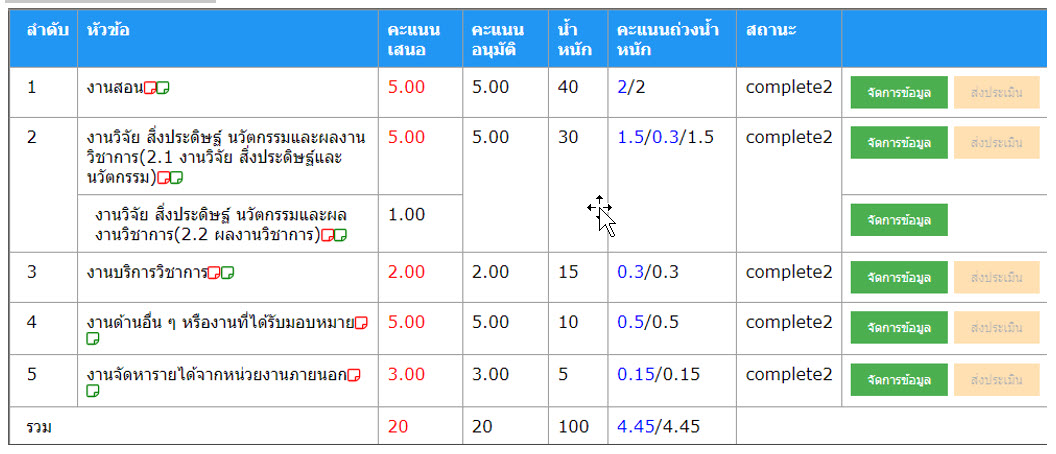
\includegraphics[width=\textwidth]{Pic5.3-1.jpg}
	\caption{ระบบประเมินสมรรถนะบุคลากรสายวิชาการ}
	\label{Pic5.3-1}
\end{figure}

โดยการประเมินสมรรถนะของบุคลากรจะอยู่ในรูปของการประเมินเพื่อเลื่อนขั้นเงินเดือนปีละ 2 ครั้ง ครั้งที่ 1 ประเมินสมรรถนะการปฏิบัติงานในช่วง 1 ตุลาคม ถึง 31 มีนาคม และครั้งที่ 2 ประเมินสมรรถนะการปฏิบัติงานในช่วง 1 เมษายน ถึง 30 กันยายน ผ่านระบบจัดการข้อมูลการประเมินบุคลากรคณะวิทยาศาสตร์และเทคโนโลยี 

นอกจากนั้นยังมีการประเมินสมรรถนะหลักของบุคลากรสายวิชาการที่กำหนดโดยมหาวิทยาลัย 6 ด้าน ประกอบไปด้วย
\begin{enumerate}
\item รักองค์กรและหน้าที่ มีจิตสำนึก ในการเป็นเจ้าของ เห็นคุณค่าองค์กร มุ่งมั่นการทำงานในหน้าที่
อย่างเป็นระบบ มีวินัยและคุณธรรมพัฒนาตนเอง และองค์กรไปสู่เป้าหมายอย่างต่อเนื่อง
\item พัฒนาตนเองเรียนรู้วิทยาการใหม่ๆ เพื่อพัฒนาและเพิ่มศักยภาพในการทำงาน ที่มีประสิทธิภาพ
และสอดคล้องต่อการ เปลี่ยนแปลง มีความรู้ ความเชี่ยวชาญ
\item เป็นมืออาชีพ มีความรู้ ความเชี่ยวชาญ ในการปฏิบัติงาน และเชื่อมโยง แก้ไขปัญหาในการทำงาน
ได้ อย่างเหมาะสมตามจรรยาบรรณวิชาชีพ
\item สื่อสารอย่างสร้างสรรค์ การถ่ายทอดข้อมูลข่าวสารโดยใช้สื่อต่างๆ มีการแลกเปลี่ยนความคิดเห็น 
และสร้างความเข้าใจร่วมกันในการทำงาน อย่างมีประสิทธิภาพเพื่อพัฒนางาน และองค์กร
\item ทำงานเป็นทีม เปิดใจกว้าง รับฟังความคิดเห็น เรียนรู้และแก้ไข ปัญหาร่วมกันอย่างมีประสิทธิภาพ 
เพื่อบรรลุเป้าหมายเดียวกัน
\item จิตสาธารณะตระหนักถึงประโยชน์ ส่วนรวมถ่ายทอดความรู้ประสบการณ์ ให้กับองค์กร สังคม
ชุมชน และประเทศชาติ
\end{enumerate}

โดยมีการกำหนดระดับสมรรถนะที่คาดหวัง ระดับสมรรถนะที่ผู้ถูกประเมินประเมินตนเอง และระดับสมรรถนะที่ประเมินโดยคณะกรรมการประเมิน ซึ่งมีคณะกรรมการ 2 ชุด คือ คณะกรรมการกลั่นกรองขั้นที่ 1 และคณะกรรมการประเมินชุดที่ 2 เป็นผู้ประเมิน รายละเอียดของข้อมูลแสดงดังภาพที่ \ref{Pic5.3-2}
\begin{figure}[h!]
	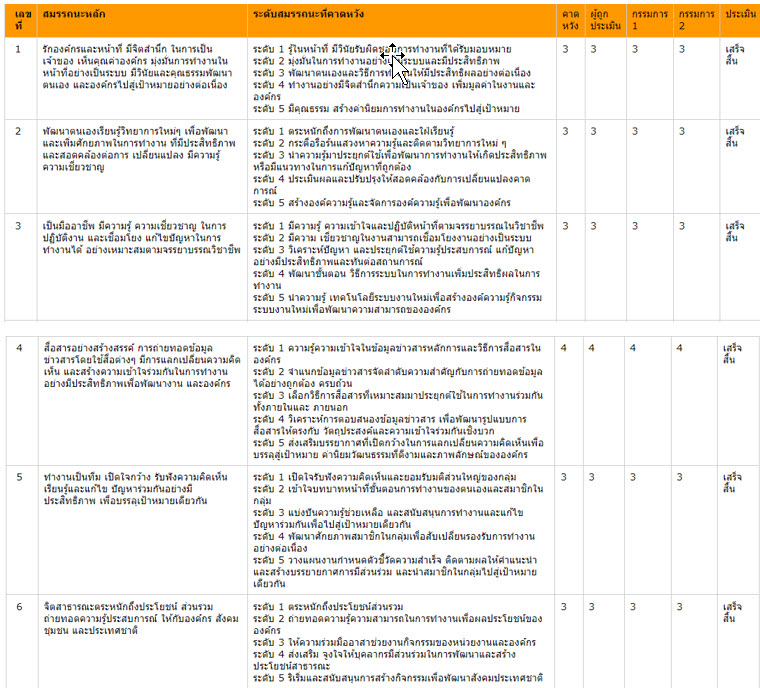
\includegraphics[width=\textwidth]{Pic5.3-2.jpg}
	\caption{สมรรถนะหลักของบุคลากรสายวิชาการที่กำหนดโดยมหาวิทยาลัย}
	\label{Pic5.3-2}
\end{figure}
รายละเอียดต่าง ๆ ในการเตรียมเอกสารและการ upload file จะมีการสื่อสารให้บุคลากรสายวิชาการได้รับทราบและเข้าใจตรงกันอย่างทั่วถึง โดยมีการสื่อสารจากการประชุมบุคลากรของคณะโดยคณบดี รองคณบดีฝ่ายบริหารและวางแผนเป็นผู้ชี้แจง ประชุมภาควิชาโดยหัวหน้าภาควิชาเป็นผู้ชี้แจง ประชุมสาขาวิชาโดยหัวหน้าสาขาวิชาเป็นผู้ชี้แจง กลุ่มบุคลากรสายวิชาการที่ถูกประเมินจะแบ่งเป็น 5 กลุ่มคือ 1) พนักงานมหาวิทยาลัยวุฒิปริญญาเอก 2) พนักงานมหาวิทยาลัยวุฒิปริญญาโท 3) ข้าราชการพลเรือน 4) ข้าราชการ (ที่เป็นผู้บริหาร) และ 5) พนักงานมหาวิทยาลัยวุฒิปริญญาเอก (ที่เป็นผู้บริหาร) นอกจากนั้นรายละเอียดการประเมินของบุคลากรสายวิชาการแต่ละกลุ่ม ขั้นตอนการประเมิน วิธีการ upload เอกสารเข้าสู่ระบบการประเมิน สามารถศึกษาคู่มือการใช้ระบบนี้ได้จากเว็บไซต์  https://sci1.rmutt.ac.th/?page\_id=22472  แสดงดังภาพที่ \ref{Pic5.3-3}\newpage

\begin{figure}[h!]
	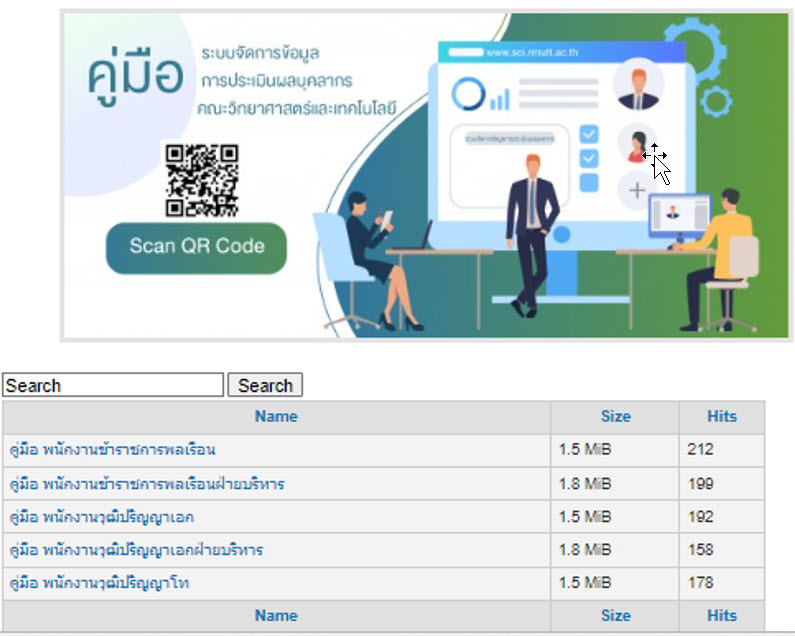
\includegraphics[width=\textwidth]{Pic5.3-3.jpg}
	\caption{คู่มือการใช้งานระบบจัดการข้อมูลการประเมินบุคลากรคณะวิทยาศาสตร์และเทคโนโลยี}
	\label{Pic5.3-3}
\end{figure}
\noindent
ขั้นตอนการประเมินสมรรถนะบุคลากรสายวิชาการ
\begin{enumerate}
\item ฝ่ายบริหารและวางแผนแจ้งบุคลากรสายวิชาการทราบถึงช่วงเวลาที่ จะต้อง upload เอกสารภาระงานตามสมรรถนะด้านต่าง ๆ ขึ้นสู่ระบบ 
\item บุคลากรสายวิชาการเตรียมเอกสารประเมินและ upload เอกสารเข้าสู่ระบบภายในเวลาที่กำหนด
\item คณะกรรมการประเมินชุดที่ 1 ที่เป็นคณะกรรมการกลั่นกรองเบื้องต้นประเมินเอกสาร 
\item คณะกรรมการเบื้องต้นแจ้ง ผลการประเมินเบื้องต้นกับบุคลากรสายวิชาการถึงคะแนนเบื้องต้น เอกสารหลักฐานครบถ้วนหรือไม่ หากเอกสารไม่ครบถ้วนมีการเปิดระบบให้ส่งเอกฐานเพิ่มเติม
\item คณะกรรมการประเมินชุดที่ 2 ประเมินผลการปฏิบัติงานต่อจากคณะกรรมการประเมินชุดที่ 1 หากมีข้อทักท้วงไม่เห็นด้วยให้ชี้แจงและส่งเอกสารแนบภายในระยะเวลาที่ระบบเปิดเท่านั้น
\item เอกสารผลการประเมินขั้นสุดท้ายส่งถึงผู้ถูกประเมิน เพื่อรับทราบและยอมรับผลการประเมิน
\end{enumerate}

ที่ผ่านมาในการประเมินผลการปฏิบัติงานของบุคลากรสายวิชาการ สาขาวิชาคณิตศาสตร์ประยุกต์ไม่มีปัญหาการฟ้องร้อง หรือการไม่ยอมรับผลการประเมิน เนื่องจากผลการประเมินยึดจากเอกสารหลักฐาน และผลการปฏิบัติงานซึ่งเป็นข้อเท็จจริงตามเกณฑ์การประเมินที่กำหนดไว้อย่างชัดเจน

\begin{doclist}
	\docitem{ระบบจัดการข้อมูลการประเมินบุคลากรคณะวิทยาศาสตร์และเทคโนโลยีออนไลน์}
\end{doclist}

%%%%%%%%%% 5.4 %%%%%%%%%%%%%%%
\subcriteria{The programme to show that the duties allocated to the academic staff are appropriate to qualifications, experience, and aptitude.}

บุคลากรสายวิชาการมีภาระหน้าที่หลัก คือ งานสอน วิจัย บริการวิชาการ และงานที่ได้รับมอบหมายทั้งในระดับสาขาวิชาและระดับคณะ 

การกำหนดผู้สอนของรายวิชา อาจารย์ผู้รับผิดชอบหลักสูตรจะพิจารณากำหนดผู้สอนรายวิชาตามความเชี่ยวชาญ ประสบการณ์การสอน ประสบการณ์การทำวิจัย โดยให้เป็นไปตามเกณฑ์ภาระงานขั้นต่ำ และกำหนดให้ผู้สอน 1 ท่าน มีจำนวนรายวิชาที่สอนไม่เกินภาคเรียนละ 3 รายวิชา

สำหรับการมอบหมายภาระงานในหลักสูตร จะพิจารณาจากความรู้ ความสามารถ ประสบการณ์ และความถนัดของอาจารย์แต่ละท่าน เช่น 
\begin{enumerate}
\item งานวิจัย มอบหมายให้ รศ.ดร.พงศกร สุนทรายุทธ์ และ ผศ.ดร.วงศ์วิศรุต เขื่องสตุ่ง เป็นผู้รับผิดชอบหลัก เนื่องจากมีประสบการณ์ในการวิจัย มีผลงานตีพิมพ์เป็นจำนวนมาก และมีประสบการณ์ในการเป็นหัวหน้าโครงการวิจัย
\item การบริหารหลักสูตร มอบหมายให้ ผศ.สมนึก ศรีสวัสดิ์ ผศ.มงคล ทาทอง ผศ.ดร.วงศ์วิศรุต เขื่องสตุ่ง รศ.ดร.พงศกร สุนทรายุทธ์ และ ดร.รัฐพรหม พรหมคำ เป็นผู้รับผิดชอบหลัก เนื่องจากเป็นอาจารย์ผู้รับผิดชอบหลักสูตร และมีประสบการณ์การบริหารหลักสูตร
\item การจัดหาสิ่งสนับสนุนการเรียนรู้ มอบหมายให้ ผศ.มงคล ทาทอง เป็นผู้รับผิดชอบหลัก เนื่องจากมีประสบการณ์ในการจัดซื้อจัดจ้าง การขอวัสดุครุภัณฑ์  
\item งานประกันคุณภาพการศึกษา มอบหมายให้ ผศ.สมนึก ศรีสวัสดิ์ ผศ.มงคล ทาทอง ผศ.ดร.วงศ์วิศรุต เขื่องสตุ่ง รศ.ดร.พงศกร สุนทรายุทธ์ และ ดร.รัฐพรหม พรหมคำ เป็นผู้รับผิดชอบหลัก เนื่องจากมีประสบการณ์การประกันคุณภาพหลักสูตร
\item งานบริการวิชาการ มอบหมายให้ ดร.รัฐพรหม พรหมคำ เป็นผู้รับผิดชอบหลัก เนื่องจากมีประสบการณ์ด้านการจัดโครงการการบริการวิชาการ
\end{enumerate}

โดยอาจารย์ผู้สอนในหลักสูตรท่านอื่น ๆ จะเป็นผู้ช่วยรับผิดชอบในแต่ละงาน และทำหน้าที่ตามพันธกิจหลักของอาจารย์ทั้ง 3 ด้านคือ สอน วิจัย และบริการวิชาการ

%%%%%%%%%% 5.5 %%%%%%%%%%%%%%%
\subcriteria{The programme to show that promotion of the academic staff is based on a merit system which accounts for teaching, research, and service.}

การขอกำหนดตำแหน่งทางวิชาการของบุคลากรสายวิชาการ มหาวิทยาลัยมีการกำหนด
ขั้นตอนการดำเนินงานการขอกำหนดตำแหน่งทางวิชาการของบุคลากรสายวิชาการ ดังนี้\\

\noindent
{\bf ส่วนของคณะ (การประเมินการสอน)}
\begin{enumerate}
\item ผู้ขอประเมินการสอน ยื่นเอกสารขอประเมินการสอน  งานบุคลากรตรวจสอบคุณสมบัติพร้อมเอกสาร
\item เสนอเรื่องไปยังคณบดี พร้อมเสนอชื่อคณะอนุกรรมการประเมินการสอน จำนวน 3 ท่าน โดย
คณะกรรมการประกอบไปด้วย \\1) คณบดี \\2) อาจารย์ในสาขาวิชาที่ขอตำแหน่งทางวิชาการ และ \\3) หัวหน้าภาควิชา/หัวหน้าสาขาวิชา
\item ตั้งอนุกรรมการประเมินการสอน 
\item นำส่งเอกสารและแบบฟอร์มการประเมินไปยังคณะอนุกรรมการประเมินการสอน
\item  รวบรวมผลการประเมินฯ ส่งมหาวิทยาลัย 
\end{enumerate}
ขั้นตอนการเสนอขอกำหนดตำแหน่งทางวิชาการ
\begin{enumerate}
\item คณะ/วิทยาลัย รับผลงานและเอกสารที่เกี่ยวข้องจากผู้เสนอขอกำหนดตำแหน่งทางวิชาการ โดยดำเนินการดังนี้
\begin{enumerate}[label=1.\arabic*,leftmargin=0.7cm, labelsep=2mm]
\item ตรวจสอบคุณสมบัติการขอกำหนดตำแหน่ง
\item ตรวจสอบเอกสารที่เกี่ยวข้องให้ครบถ้วน
\item แต่งตั้งคณะอนุกรรมการประเมินการสอนและประเมินเอกสารตามตำแหน่งทางวิชาการ
\item ดำเนินการให้คณะอนุกรรมการประเมินการสอนและประเมินเอกสารฯให้แล้วเสร็จและผ่าน
การประเมิน
\end{enumerate}
\item คณะ/วิทยาลัย ดำเนินการทำหนังสือส่งพร้อมรวบรวมผลงาน  เอกสารที่เกี่ยวข้อง คำสั่งแต่งตั้งอนุกรรมการ  ผลการประเมินการสอน ส่งกองบริหารงานบุคคล
\item กองบริหารงานบุคคลตรวจสอบคุณสมบัติ ผลงานทางวิชาการและเอกสารที่เกี่ยวข้อง ตามกรณีดังนี้
\begin{enumerate}[label=3.\arabic*,leftmargin=0.7cm, labelsep=2mm]
\item คุณสมบัติและผลงานไม่เป็นไปตามเกณฑ์ที่ ก.พ.อ.กำหนด ส่งเรื่องคืนคณะ/วิทยาลัย
\item เอกสารที่เกี่ยวข้องไม่ถูกต้อง ไม่ครบถ้วน แจ้งผู้เสนอขอให้นำกลับไปแก้ไข
\end{enumerate}
\item นำเข้าการประชุมคณะกรรมการกลั่นกรองผลงานทางวิชาการ เพื่อกลั่นกรองผลงานทางวิชาการเบื้องต้น
\item นำเข้าประชุมคณะกรรมการพิจารณาตำแหน่งทางวิชาการ เพื่อพิจารณาการเสนอขอและเลือกสรรผู้ทรงคุณวุฒิ ผู้ประเมินผลงานทางวิชาการ
\item ทาบทามผู้ทรงคุณวุฒิเพื่อทำหน้าที่ประเมินผลงานทางวิชาการจริยธรรมและจรรยาบรรณทางวิชาการ
\item ส่งผลงานให้ผู้ทรงคุณวุฒิประเมินผลงานทางวิชาการ
\item ประชุมคณะกรรมการผู้ทรงคุณวุฒิประเมินผลงานทางวิชาการเพื่อสรุปผลการประเมินผลงานทางวิชาการ
\item นำเข้าการประชุมคณะกรรมการพิจารณาตำแหน่งทางวิชาการ โดยหากมีมติปรับปรุงผลงาน ดำเนินการตามขั้นตอน ข้อที่ 9.1 - 9.3 หากไม่มีการปรับปรุงผลงานทำตามขั้นตอนข้อที่ 10
\begin{enumerate}[label=9.\arabic*,leftmargin=0.7cm, labelsep=2mm]
\item หากมีมติให้ปรับปรุงผลงาน กองบริหารงานบุคคลแจ้งต้นสังกัดให้ผู้เสนอขอฯปรับปรุงผลงาน 
ตามกำหนดเวลา
\item เมื่อผู้เสนอขอปรับปรุงผลงานแล้วเสร็จ กองบริหารงานบุคคลนำส่งผลงานปรับปรุงให้
ผู้ทรงคุณวุฒิประเมิน ผลงานปรับปรุง
\item เมื่อผู้ทรงคุณวุฒิฯประเมินผลงานปรับปรุงแล้วเสร็จ จึงนำเข้าการประชุมคณะกรรมการ
พิจารณาตำแหน่ง ทางวิชาการ
\end{enumerate}
\item นำเข้าการประชุมสภามหาวิทยาลัยเพื่อพิจารณาผลการขอกำหนดตำแหน่งทางวิชาการ
\item แจ้งผลการขอกำหนดตำแหน่งทางวิชาการไปยังต้นสังกัด โดยรอมติสภามหาวิทยาลัยเพื่อดำเนินการดังนี้
\begin{enumerate}[label=11.\arabic*,leftmargin=0.8cm, labelsep=2mm]
\item กรณีอนุมัติ ส่งคำสั่งแต่งตั้งและการ์ดแสดงความยินดีไปยังคณะ/
วิทยาลัย
\item กรณีไม่อนุมัติ แจ้งเรื่องและรายละเอียดการไม่อนุมัติไปยังคณะ/วิทยาลัย
\end{enumerate}
\end{enumerate}

 หลักสูตรมีกระบวนการส่งเสริมการเข้าสู่ตำแหน่งทางวิชาการโดยให้อาจารย์ทุกท่านจัดทำแผนการเสนอขอกำหนดตำแหน่งทางวิชาการ จัดระบบพี่เลี้ยงให้คำแนะนำปรึกษาและกำกับติดตาม ส่งผลให้
ในปีการศึกษา 2567 มีอาจารย์ผู้รับผิดชอบหลักสูตรได้ตำแหน่งทางวิชาการในตำแหน่งรองศาสตราจารย์ จำนวน 1 คน 
นอกจากนี้ยังมีอาจารย์ผู้สอนได้ตำแหน่งทางวิชาการในตำแหน่งผู้ช่วยศาสตราจารย์อีก 1 คน ปัจจุบันในหลักสูตร
มีอาจารย์ที่มีตำแหน่งทางวิชาการจำนวน 8 คน จาก 18 คน คิดเป็นร้อยละ 44.44

หลักสูตรให้ความสำคัญกับการประเมินผลตามระบบคุณธรรมที่ครอบคลุมทุกด้าน ทั้งด้านการสอน งานวิจัย และการบริการวิชาการต่อสังคม เพื่อให้การพัฒนาและความก้าวหน้าของบุคลากรเป็นไปอย่างรอบด้านและมีประสิทธิภาพ นอกจากการประเมินตามเกณฑ์มาตรฐานแล้ว มีค่าตอบแทนจากการตีพิมพ์บทความวิจัยในฐานข้อมูลระดับนานาชาติ และฐานข้อมูลระดับชาติ รวมถึงพัฒนาทักษะทางวิชาการในลักษณะต่างๆ ทั้งในประเทศและต่างประเทศ โดยค่าสมนาคุณการตีพิมพ์บทความวิจัยในวารสารระดับนานาชาติให้ใช้ค่าควอไทล์ที่ปรากฎใน
ฐานข้อมูลการจัดอันดับวารสาร Scopus โดยพิจารณาจากปีล่าสุดที่ปรากฎอยู่ในฐานข้อมูล ณ
วันที่บทความได้รับการตีพิมพ์ ดังนี้
\begin{enumerate}
	\item Top 10 \%\ หรือ Tier 1 สนับสนุน 60,000 บาท
	\item ควอไทล์ที่ 1 (Q1) สนับสนุน 30,000 บาท
	\item ควอไทล์ที่ 2 (Q2) สนับสนุน 20,000 บาท
	\item ควอไทล์ที่ 3 (Q3) สนับสนุน 10,000 บาท
	\item ควอไทล์ที่ 4 (Q4) สนับสนุน 8,000 บาท
	\item ไม่มีควอไทล์ สนับสนุน 4,000 บาท
\end{enumerate}
ส่วนหลักเกณฑ์การจ่ายเงิน และรางวัลสนับสนุนการตีพิมพ์บทความวิจัย กรณีตีพิมพ์ในวารสารระดับชาติ ค่าสมนาคุณการตีพิมพ์บทความวิจัยในวารสารระดับชาติที่อยู่ในฐานข้อมูล TCI กลุ่ม 1 หรือ กลุ่ม 2 จ่ายเงินค่าสมนาคุณการตีพิมพ์บทความวิจัย 4,000 บาท เพื่อกระตุ้นให้บุคลากรมีความมุ่งมั่นในการพัฒนาตนเองและสร้างผลงานที่สอดคล้องกับเป้าหมายของหลักสูตรอย่างต่อเนื่อง

% ดังตารางแสดงการตีพิมพ์บทความวิจัยในฐานข้อมูลระดับนานาชาติ และฐานข้อมูลระดับชาติของบุคลาการสายวิชาการ สาขาวิชาคณิตศาสตร์ประยุกต์ ประจำปีการศึกษา 2567 
%{\small
%\begin{longtable}{|p{0.3\textwidth}|>{\raggedright}p{0.2\textwidth}|>{\raggedright}p{0.2\textwidth}|>{\raggedright}p{0.05\textwidth}|p{0.07\textwidth}|}
%	\caption{การตีพิมพ์บทความวิจัยในฐานข้อมูลระดับนานาชาติ และฐานข้อมูลระดับชาติ}
%	\label{table: Teacher-Develop}
%	\\
%	\hline
%	\centering\textbf{ชื่อ-สกุล}&\centering\textbf{ชื่อผลงาน}&\centering\textbf{แหล่งเผยแพร่/ตีพิมพ์}
%	&\centering\textbf{ปีที่ตีพิมพ์}&\textbf{ฐาน\newline ข้อมูล}\\\hline
%	\endfirsthead
%	\caption[]{(ต่อ) การตีพิมพ์บทความวิจัยในฐานข้อมูลระดับนานาชาติ และฐานข้อมูลระดับชาติ}
%	\\
%	\hline
%	\centering\textbf{ชื่อ-สกุล}&\centering\textbf{ชื่อผลงาน}&\centering\textbf{แหล่งเผยแพร่/ตีพิมพ์}
%&\centering\textbf{ปีที่ตีพิมพ์}&\textbf{ฐาน\newline ข้อมูล}\\\hline
%	\endhead
%	
%	1. นายสมนึก ศรีสวัสดิ์	
%	&1. Some identities of (s, t)-Pell and (s, t)-Pell-Lucas polynomials by matrix methods
%	&International Journal of Mathematics and Computer Science	
%	&2024
%	&Scopus\newline Q2\\
%	\cline{2-5} 
%	&2. Novel inertial methods for fixed point problems in reflexive Banach spaces with applications	
%	&Rendiconti del Circolo Matematico di Palermo Series 2	
%	&2024	
%	&Scopus\newline Q1\\
%	\hline
%	%==================================================
%	2. นายพงศกร สุนทรายุทธ์
%	&1. Three novel inertial subgradient extragradient methods for quasi-monotone variational inequalities in Banach spaces	&Computational and AppliedMathematics	
%	&2024	
%	&Scopus\newline Q1\\
%	\cline{2-5}
%	&2. Novel inertial methods for fixed point problems in reflexive Banach spaces with applications	
%	&Rendiconti del Circolo Matematico di Palermo Series 2	
%	&2024	
%	&Scopus\newline Q1\\
%	\cline{1-5}
%	&3. Modified accelerated Bregman projection methods for solving quasimonotone variational inequalities	
%	&Optimization	
%	&2024	
%	&Scopus\newline Q1\\
%	\hline
%%==================================================
%	3. นายวงศ์วิศรุต เขื่องสตุ่ง
%	&1. Some New Results on Fixed Points for 𝜛-Distances in Complex-Valued Metric Spaces	
%	&Science and Technology Asia	
%	&2024	
%	&Scopus\newline Q4\\
%	\cline{2-5}
%	&2. A Modified Krasnoselskii-type Subgradient Extragradient Algorithm with Inertial Effects for Solving Variational Inequality Problems and Fixed Point Problem	
%	&Nonlinear Functional Analysis and Applications	
%	&2024	
%	&Scopus\newline Q2\\
%	\cline{2-5}
%	&3. A Regularization Method for Solving the G-Variational Inequality Problem and Fixed-Point Problems in Hilbert Spaces Endowed with Graphs	
%	&Journal of Inequalities and Applications	
%	&2024	
%	&Scopus\newline Q1\\
%	\cline{1-5}
%	&4. Self-adaptive CQ-type Algorithms for the Split Feasibility Problem Involving Two Bounded Linear Operators in Hilbert Spaces	
%	&Carpathian Journal of Mathematics	
%	&2024	
%	&Scopus\newline Q1\\
%	\hline
%	%=================================================
%	4. นายรัฐพรหม พรหมคำ
%	&1. Three novel inertial subgradient extragradient methods for quasi-monotone variational inequalities in Banach spaces	&Computational and Applied Mathematics
%	&2024	
%	&Scopus\newline Q1\\
%	\cline{2-5}
%	&2. Novel inertial methods for fixed point problems in reflexive Banach spaces with applications	
%	&Rendiconti del Circolo Matematico di Palermo Series 2	
%	&2024	
%	&Scopus\newline Q1\\
%	\hline
%	%==============================================
%	5. นายมงคล ทาทอง
%	&1. Some Matrices with Padovan Q-matrix and the Generalized Relations	
%	&Progress in Applied Science and Technology	
%	&2024	
%	&TCI1\\
%	\hline
%	%==============================================
%	6. นางวรรณา ศรีปราชญ์
%	&1. Some identities of (s,t)-Pell and (s, t)-Pell-Lucas polynomials by matrix methods	
%	&International Journal of Mathematics and Computer Science	
%	&2024	
%	&Scopus\newline Q2\\
%	\hline
%	%==============================================
%	7. นายปริญญวัฒน์ ชูสุวรรณ
%	&1.Generalized Order Divisor of Finite Groups
%	&International Journal of Group Theory	
%	&2024	
%	&Scopus\newline Q3\\
%	\hline
%	%==============================================
%	8. นางสาวปฤณท์ธพร\newline สงวนสุทธิกุล 
%	&A Bilevel QP-PLP Approach to Demand Response Modulation between Consumers and a Single Electricity Seller	
%	&Science and Technology Asia	
%	&2024	
%	&Scopus\newline Q3\\
%	\hline
%	%===============================================
%	9. นางสาวนนธิยา มากะเต
%	&1.Bi-Periodic k-Pell Sequence
%	&International Journal of Mathematics and Computer Science	
%	&2024	
%	&Scopus\newline Q2\\
%	\hline
%	%===============================================
% 10. นางสาวกมลรัตน์ สมบุตร
%	&1. Best Proximity Points of Generalized Geraghty Proximal Contractions in Generalized Metric Spaces	
%	&Fixed Point Theory	
%	&2024	
%	&Scopus\newline Q2\\
%	\cline{2-5}
%	&2. Existence and Uniqueness of Solutions of a Coupled System of  ψ-Hilfer Fractional Differential Equations under Uncoupled Non-Local Multi Point Conditions Involving Fixed Point Theorems	
%	&J. Nonlinear Funct. Anal.	
%	&2024	
%	&Scopus\newline Q3\\
%	\hline
%%=================================================
%11. นายอัคเรศ สิงห์ทา
%&1.  A regularization method for solving the G-variational inequality problem and fixed-point problems in Hilbert spaces endowed with graphs	&Journal of Inequalities and Applications	
%&2024	
%&Scopus\newline Q1\\
%\hline
%%================================================
%12. นางภคีตา สุขประเสริฐ
%	&1. Ciric-contraction type via wt-distance	
%	&Advances in Fixed Point Theory	
%	&2024	
%	&Scopus\newline Q4\\
%	\cline{2-5}
%	&2. A SPECTRAL CLASS OF DAI-KOU-TYPE METHODS WITH APPLICATIONS TO SIGNAL PROCESSING	
%	&Journal of Nonlinear Functional Analysis	
%	&2024	
%	&Q1\\
%	\hline
%	%================================================
%	13. นางสาววาสนา ทองกำแหง
%	&1. Pseudo N Q-principally Projective Modules	
%	&International Journal of Mathematics and Computer Science	
%	&2024	
%	&Scopus\newline Q2\\
%	\hline
%	%================================================
%	14. นางสาวอมราภรณ์ บำเพ็ญดี
%	&1. Pseudo N Q-principally Projective Modules	
%	&International Journal of Mathematics and Computer Science	
%	&2024	
%	&Scopus\newline Q2\\
%	\hline	
%\end{longtable}}
\begin{doclist}
	\docitem{เว็บไซต์ของมหาวิทยาลัยที่ให้ข้อมูลเกี่ยวกับการเข้าสู่ตำแหน่งทางวิชาการ https://www.ped.rmutt.ac.th/?p=4552}
	\docitem{เว็บไซต์ของมหาวิทยาลัยที่ให้ข้อมูลเกี่ยวกับระบบบริหารข้อมูลงานวิจัยและงานบริการวิชาการ https://sciresearch-rmutt.com/ResDocs}
\end{doclist}
%%%%%%%%%% 5.6 %%%%%%%%%%%%%%%
\subcriteria{The program to show that the rights and privileges, benefits, roles and relationships, and accountability of the academic staff, taking into account professional ethics and their academic freedom, are well defined and understood.}
สาขาวิชาคณิตศาสตร์ประยุกต์มีบุคลาการสายวิชาการจำนวน 18 คน เป็นพนักงานมหาวิทยาลัยจำนวน 18 คน  โดยบุคลากรสายวิชาการทุกท่านรับทราบสวัสดิการและสิทธิประโยชน์ต่างๆ มหาวิทยาลัยโดย กองบริหารงานบุคคล จะแจ้งข้อมูลเหล่านี้ผ่านทางงานบุคลากรของคณะและแจ้งผ่านเว็บไซต์ของมหาวิทยาลัย  https://www.rmutt.ac.th/welfare-for-personnel/ 
\begin{figure}[h!]
	\begin{center}
	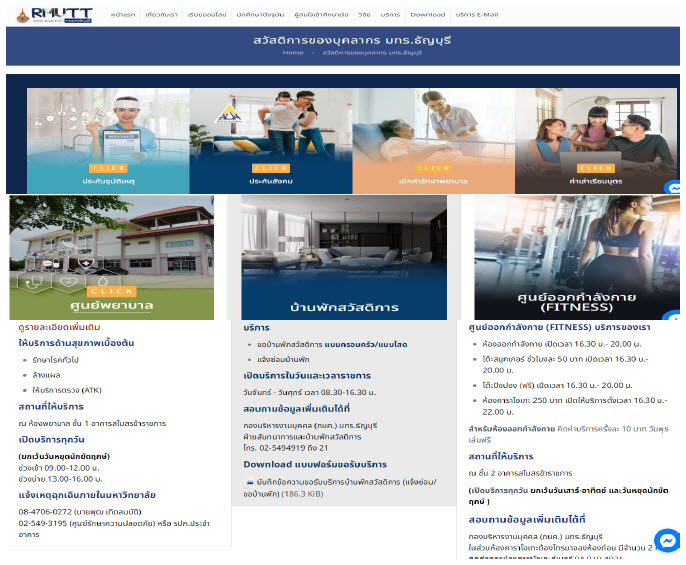
\includegraphics[width=0.6\textwidth]{Pic5.6-1.jpg}
	\caption{สวัสดิการของบุคลากร มทร.ธัญบุรี}
	\label{Pic5.6-1}
	\end{center}
\end{figure}

\newpage
นอกจากนั้นในส่วนของมหาวิทยาลัยมีการจัดสวัสดิการที่เกี่ยวข้องกับการส่งเสริมสุขภาพที่ดี ประกอบด้วย
โครงการตรวจสุขภาพประจำปี สโมสร ศูนย์ออกกำลังกาย สระว่ายน้ำ สนามกีฬา การแข่งขันกีฬาบุคลากร และมีการสร้างขวัญและกำลังใจเพื่อให้บุคลากรทำงานได้อย่างมีประสิทธิภาพประสิทธิผล ประกอบด้วย การจัดทำประกันอุบัติเหตุให้กับบุคลากร เงินช่วยเหลือบุตร เงินช่วยเหลือค่าทำศพ บ้านพักสวัสดิการบุคลากร รางวัลบุคลากรดีเด่น การให้บุคลากรไปฝึกอบรมพัฒนาศึกษาดูงานทั้งในประเทศ/ต่างประเทศ นอกจากนี้คณะฯ ยังมีการจัดสวัสดิการและสิ่งจูงใจเพิ่มเติมนอกเหนือจากที่มหาวิทยาลัยจัดให้ดังนี้    
\begin{itemize}   
\item มีการประกาศยกย่องผู้ที่ได้ทำชื่อเสียงให้แก่คณะผ่านทางเว็บไซต์ของคณะฯ  
\item มีการจัดห้องออกกำลังกายให้กับบุคลากร 
\item มีการมอบของขวัญให้กับบุคลากรในวันขึ้นปีใหม่  
\item มีการปรับปรุงภูมิทัศน์ เพื่อส่งเสริมบรรยากาศที่ดีในการทำงาน
ในส่วนของสาขาวิชาคณิตศาสตร์ประยุกต์มีการสร้างแรงจูงใจและสวัสดิการให้แก่บุคลากรในสาขาวิชา ดังนี้
\item มีการประกาศยกย่องผู้ที่ได้ทำชื่อเสียงให้แก่สาขาวิชา ผ่านทางเว็บไซต์ของสาขาวิชา
\item มีการจัดหาสิ่งอำนวยความสะดวกในการดำรงชีพ เช่น ตู้เย็น ไมโครเวฟ เครื่องทำน้ำเย็น เครื่องทำ     น้ำร้อน น้ำดื่ม เครื่องชงกาแฟ ฯลฯ บริการแก่บุคลากรในสาขาวิชา
\item มีการจัดหาสิ่งอำนวยความสะดวกในการปฏิบัติงาน เช่น คอมพิวเตอร์ WIFI เครื่องพิมพ์ เครื่องถ่ายเอกสาร ฯลฯ บริการแก่บุคลากรในสาขาวิชานอกเหนือจากที่คณะจัดสรรให้
\item สาขาวิชามีการจัดเตรียมหนังสือ ตำรา ที่เกี่ยวข้องกับวิชาการ วิชาชีพ เพื่อบริการแก่บุคลากรในสาขาวิชา
\end{itemize}

ในส่วนของบทบาทหน้าที่ ความรับผิดชอบของอาจารย์ รวมทั้งจรรยาบรรณบุคลากร คณะและมหาวิทยาลัยมีการกำหนดแนวปฏิบัติต่างๆ รวมทั้งใช้แนวปฏิบัติของ สป.อว. เป็นกรอบดำเนินการ โดยมีการสื่อสารผ่านหัวหน้าสาขาวิชา มีการอบรมอาจารย์ใหม่ และมีข้อมูลรายละเอียดในเว็บไซต์ https://sci1.rmutt.ac.th/?page\_id=10368  เพื่อให้บุคลากรได้รับทราบตามแนวปฏิบัติ

\begin{figure}[h!]
	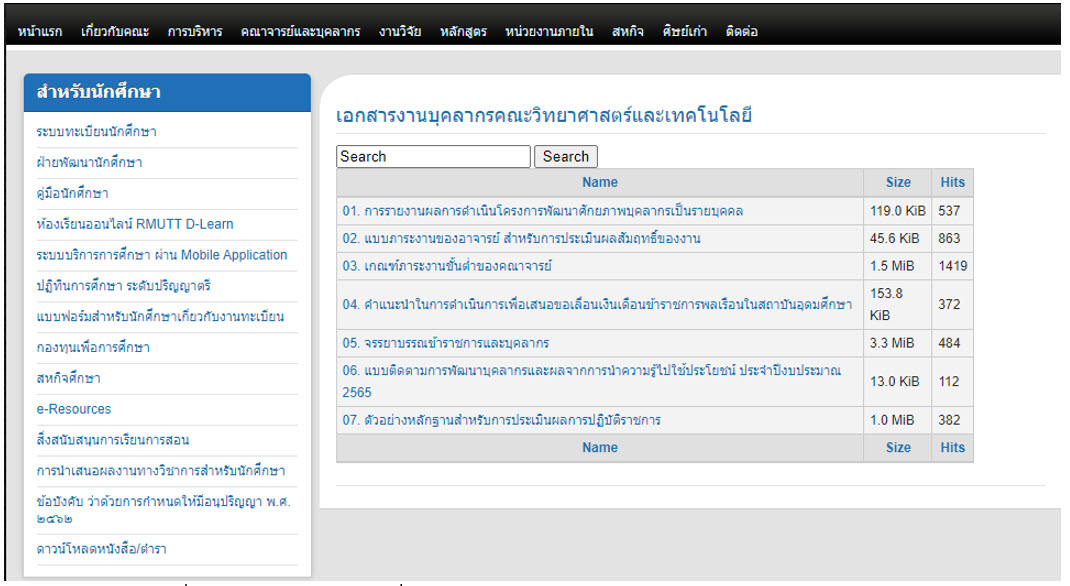
\includegraphics[width=\textwidth]{Pic5.6-2.jpg}
	\caption{บทบาทหน้าที่ความรับผิดชอบของอาจารย์และจรรยาบรรณบุคลากร}
	\label{Pic5.6-2}
\end{figure}
ในส่วนของความเป็นอิสระทางวิชาการ คณะและมหาวิทยาลัยได้ใช้แนวทางของ สป.อว. ตามประกาศเรื่องแนวปฏิบัติตามหลักความรับผิดชอบต่อสังคม หลักเสรีภาพทางวิชาการ หลักความเป็นอิสระ และหลักความเสมอภาค โดยทางหลักสูตร ได้แจ้งให้คณาจารย์ของหลักสูตรได้รับทราบผ่านการประชุมของหลักสูตร/อาจารย์ประจำสาขาวิชา
\begin{doclist}
	\docitem{เว็บไซต์คณะ : บทบาทหน้าที่ ความรับผิดชอบของอาจารย์\newline รวมทั้งจรรยาบรรณบุคลากร \newline https://sci1.rmutt.ac.th/?page\_id=10368}
	\docitem{ราชกิจจานุเบกษา แนวปฏิบัติตามหลักความรับผิดชอบต่อสังคม\newline หลักเสรีภาพทางวิชาการหลักความเป็นอิสระ และหลักความ\newline เสมอภาค}
\end{doclist}

%%%%%%%%%% 5.7 %%%%%%%%%%%%%%%
\subcriteria{The program to show that the training and developmental needs of the academic staff are systematically identified, and that appropriate training and development activities are implemented to fulfil the identified needs.}
นโยบายการพัฒนาบุคลากรด้านการฝึกอบรมของคณะฯ มุ่งเน้นไปที่ในแต่ละปีบุคลากรจะต้องพัฒนาตนเองตามสาขาวิชาชีพ และการพัฒนาตนเองตามยุทธศาสตร์ซึ่งจัดในภาพรวมที่จัดโดยคณะและมหาวิทยาลัย ในส่วนของคณะมีงบประมาณ 1,500 บาท/คน สำหรับให้บุคลากรพัฒนาตนเองตามวิชาชีพ ในส่วนของมหาวิทยาลัยมีงบประมาณจากงบพัฒนาบุคลากร 5,000 บาท/คนสำหรับจัดในภาพรวม ในแต่ละปีการศึกษามีกระบวนการในการดำเนินการพัฒนาบุคลากรด้านการฝึกอบรม  ดังนี้

\begin{figure}[h!]
	\begin{center}
	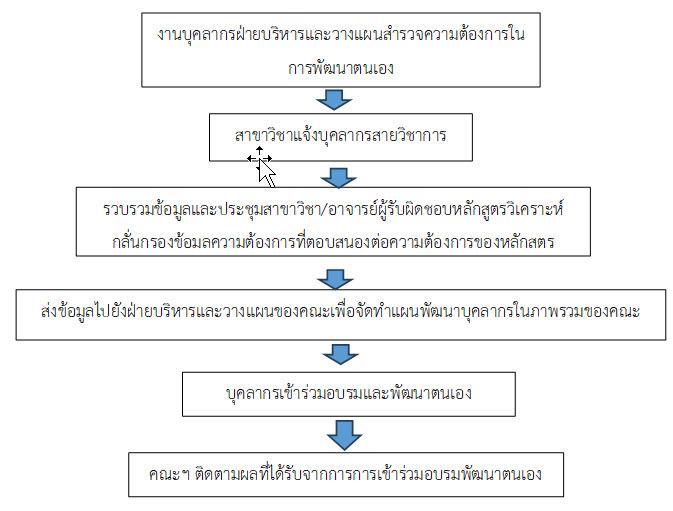
\includegraphics[width=0.8\textwidth]{Pic5.7-1.jpg}
	\caption{กระบวนการพัฒนาบุคลากรด้านการฝึกอบรมพัฒนาตนเองของคณะ}
	\label{Pic5.7-1}
	\end{center}
\end{figure}
\newpage
หลักสูตรได้ดำเนินการวางแผนเพื่อพิจารณาความต้องการที่จำเป็นของอาจารย์ภายในหลักสูตรอย่างเป็นระบบ โดยมีการร่วมกันกำหนดแนวทางในการพัฒนาคณาจารย์ให้สอดคล้องกับเป้าหมายของหลักสูตร การวางแผนดังกล่าวอ้างอิงจากข้อมูลและข้อเสนอแนะของอาจารย์ผู้สอน รวมถึงผลการประเมินตนเอง ผลการประเมินการสอน และแนวโน้มการเปลี่ยนแปลงทางวิชาการในแต่ละช่วงเวลา ซึ่งช่วยให้สามารถจัดกิจกรรมพัฒนาบุคลากรได้อย่างตรงจุดและมีเป้าหมายชัดเจน ทั้งในระดับรายบุคคลและระดับภาพรวมของหลักสูตร ความร่วมมือภายในของคณาจารย์ในกระบวนการนี้ ยังเอื้อต่อการพัฒนาอย่างเป็นระบบและต่อเนื่อง ซึ่งส่งผลดีต่อคุณภาพของการจัดการเรียนการสอน 
ทั้งนี้หลักสูตรมีการประชุมจัดทำแผนการฝึกอบรม/พัฒนาบุคลากรสายวิชาการ เพื่อให้สอดคล้องกับความต้องการของหลักสูตร โดยให้อาจารย์ทุกท่านเข้ารับการฝึกอบรมทางด้านวิชาการ/วิชาชีพทางด้านคณิตศาสตร์หรือคณิตศาสตร์ประยุกต์อย่างน้อยปีละ 1 ครั้ง พร้อมทั้งรายงานผลการฝึกอบรมและการนำไปใช้ให้หลักสูตรทราบ


ในปีการศึกษา 2567  เนื่องจากหลักสูตรจะมีการประเมินคุณภาพหลักสูตรตามเกณฑ์มาตรฐาน AUN-QA จึงเพิ่มข้อกำหนดให้อาจารย์ทุกท่านเข้ารับการอบรม/พัฒนาตนเองด้านการประกันคุณภาพหลักสูตรตามเกณฑ์มาตรฐาน AUN-QA และจัดทำเป็นแผนให้อาจารย์ทุกท่านพัฒนาตนเอง ดังนี้
\begin{enumerate}
	\item ด้านวิชาการ/วิชาชีพทางด้านคณิตศาสตร์หรือคณิตศาสตร์ประยุกต์อย่างน้อยปีละ 1 ครั้ง
	\item ด้านการประกันคุณภาพหลักสูตรตามเกณฑ์มาตรฐาน AUN-QA อย่างน้อย 1 ครั้ง
\end{enumerate}

ผลการดำเนินงานในปีการศึกษา 2567 อาจารย์ทุกท่านเข้ารับการอบรม/พัฒนาตนเอง ตามแผนที่กำหนด รายละเอียดดังตาราง \ref{table: Teacher-Develop}

\begin{longtable}{|>{\raggedright}p{0.45\textwidth}|>{\raggedright}p{0.2\textwidth}|p{0.2\textwidth}|}
	\caption{โครงการพัฒนาบุคลากรที่อาจารย์ทุกท่านในหลักสูตรเข้าร่วมในปีการศึกษา 2567}
	\label{table: Teacher-Develop}
	\\
	\hline
\centering\textbf{หัวข้อที่เข้าอบรม}&\centering\textbf{วันที่}
&\multicolumn{1}{c|}{\textbf{หน่วยงานที่จัด}}
\\
\hline
	\endfirsthead
	\caption[]{(ต่อ) การพัฒนาตนเองของบุคลาการสายวิชาการ สาขาวิชาคณิตศาสตร์}
	\\
	\hline
\textbf{หัวข้อที่เข้าอบรม}&\textbf{วันที่}
&\textbf{หน่วยงานที่จัด}\\
	\hline
	\endhead

โครงการอบรมการประกันคุณภาพการศึกษาระดับหลักสูตรตามเกณฑ์ AUN-QA(ASEAN University Network Quality Assurance:AUN-QA) 	
&20-21 พฤษภาคม 2568 	
&คณะวิทยาศาสตร์และเทคโนโลยี\\
\hline
โครงการพัฒนาศักยภาพบุคลากรสาขาคณิตศาสตร์เพื่อเตรียมความพร้อมทางด้านวิทยาการข้อมูล
& 2-3 มิถุนายน 2568	
&สาขาวิชาคณิตศาสตร์ \\
\hline
 
\end{longtable}
นอกจากนี้อาจารย์ในหลักสูตรยังได้เข้ารับการอบรมพัฒนาตนเองในหัวข้ออื่นๆ ตามความสนใจ และสอดคล้องกับแนวทางในการส่งเสริมพัฒนาบุคลากรของหลักสูตร
\begin{doclist}
	\docitem{แผนพัฒนาตนเองรายบุคคล (IDP) ปีการศึกษา 2567}
\end{doclist}
\newpage
%%%%%%%%%% 5.8 %%%%%%%%%%%%%%%
\subcriteria{The program to show that performance management including reward and recognition is implemented to assess academic staff teaching and research quality.}

หลักสูตรวิทยาศาสตรบัณฑิต สาขาวิชาคณิตศาสตร์ประยุกต์ ใช้แนวทางการประเมินผลการปฏิบัติงานของอาจารย์ตามระบบจัดการข้อมูลการประเมินบุคลากรคณะวิทยาศาสตร์และเทคโนโลยีโดยจะประเมิน 2 ครั้ง ครั้งที่ 1 คือ 1 ตุลาคม ถึง 31 มีนาคม และ
ครั้งที่ 2 คือ 1 เมษายน ถึง 30 กันยายน
 โดยคะแนนประเมินจะมาจาก 2 ส่วนประกอบคือ 
\begin{enumerate}
\item ภาระงานด้านการเรียนการสอน วิจัย การบริการทางวิชาการ งานมอบหมายอื่น ๆ และการหารายได้ คิดเป็นสัดส่วนคะแนน 70\%
\item ประเมินสมรรถนะหลักของบุคลากรสายวิชาการที่กำหนดโดยมหาวิทยาลัย 6 ด้าน คิดเป็นสัดส่วนคะแนน 30\%
\end{enumerate}

เมื่อบุคลากรสายวิชาการเนินการประเมินผลงานเรียบร้อยแล้ว  จะมีการแจ้งผลการประเมินเพื่อสะท้อนให้เห็นผลการปฏิบัติงาน และผู้ถูกประเมินรับทราบผลการประเมินเพื่อนำผลการประเมินนำไปปรับปรุงในรอบถัดไป หลังจากนั้นคณะนำเสนอข้อมูลไปยังมหาวิทยาลัย เพื่อพิจารณาอนุมัติการขึ้นเงินเดือน และจะมีการแจ้งผลการขึ้นเงินเดือนของแต่ละรายบุคคลผ่านเว็บไซต์ www.hr.rmutt.ac.th โดยบุคลากรสายวิชาการแต่ละคนต้อง log in ด้วย username และ password ของตนเอง

มีการสร้างขวัญกำลังใจ การยกย่องเชิดชูเกียรติ การให้รางวัล ทั้งของระดับหลักสูตรฯ ระดับคณะฯ และระดับมหาวิทยาลัย 

ในส่วนของระดับคณะฯ และหลักสูตรฯ มีการแสดงยินดีผ่าน Web-site/Facebook ของคณะฯ และสาขาวิชาฯ ซึ่ง
ในปีการศึกษา 2567 มีบุคลากรสายวิชาการของสาขาวิชาที่ได้ตำแหน่งทางวิชาการในตำแหน่งรองศาสตราจารย์ จำนวน 1 คน 
 คือ ผศ.ดร.วงศ์วิศรุต เขื่องสตุ่ง นอกจากนี้ยังมีอาจารย์ผู้สอนได้ตำแหน่งทางวิชาการในตำแหน่งผู้ช่วยศาสตราจารย์อีก 1 คน คือ ผศ.ดร.วรรณา ศรีปราชญ์ และได้มีการแสดงความยินดีผ่าน website และ Facebook ดังภาพที่ \ref{Pic5.8-1}
\begin{figure}[h!]
	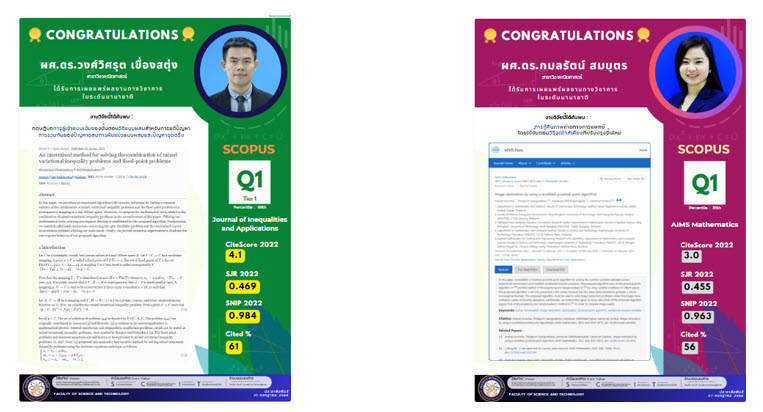
\includegraphics[width=\textwidth]{Pic5.8-1.jpg}
	\caption{บุคลากรของสาขาวิชาที่ได้รับการแต่งตั้งให้ดำรงตำแหน่งทางวิชาการปีการศึกษา 2567}
	\label{Pic5.8-1}
\end{figure}

นอกจากนี้ในระดับมหาวิทยาลัยยังมีการให้เงินรางวัล ทางด้านรางวัลสำหรับอาจารย์ที่มีผลงานวิจัยเผยแพร่รายละเอียดดังตารางที่ \ref{Table:award}
\begin{center}
		\begin{longtable}{|p{0.55\textwidth}|p{0.4\textwidth}|}
			 \caption{อัตราเงินรางวัลสำหรับอาจารย์ที่เผยแพร่ผลงานทางวิชาการ}
			\label{Table:award}\\
			\hline
		   \textbf{รูปแบบการเผยแพร่ผลงานทางวิชาการ}	&\textbf{เงินรางวัล/ผลงาน (บาท)}\\
		  	 \hline
			\endfirsthead
			 \caption{(ต่อ) อัตราเงินรางวัลสำหรับอาจารย์ที่เผยแพร่ผลงานทางวิชาการ}
		\\
		\hline
		\textbf{รูปแบบการเผยแพร่ผลงานทางวิชาการ}	&\textbf{เงินรางวัล/ผลงาน (บาท)}\\
		\hline
		\endhead	
			%%%%%%%%%%%%%%%%%%%%%%%%%%
			\multicolumn{2}{|l|}{\textbf{วารสารวิชาการระดับชาติ}	
		}\\
			\hline
			ค่าสมนาคุณการตีพิมพ์บทความวิจัยในวารสารระดับชาติที่อยู่ในฐานข้อมูล TCI กลุ่ม 1 หรือ กลุ่ม 2	&4,000 บาท\\
			\hline
			ค่าธรรมเนียมการตีพิมพ์บทความวิจัย (Page   charge) ของวารสารที่อยู่ในฐานข้อมูล TCI      	&ตามที่จ่ายจริงแต่ไม่เกิน  5,000 บาท\\
			\hline
			\multicolumn{2}{|l|}{\textbf{วารสารวิชาการระดับนานาชาติ}}\\
			\hline
			ค่าสมนาคุณการตีพิมพ์บทความวิจัย Scopus Top 10% หรือ Tier 1
			&60,000 บาท\\
			\hline
			ค่าสมนาคุณการตีพิมพ์บทความวิจัยควอไทล์ที่ 1 (Q1)         	&30,000 บาท	\\
			\hline
			ค่าสมนาคุณการตีพิมพ์บทความวิจัย ควอไทล์ที่ 2 (Q2)         	&20,000 บาท	\\
			\hline
			ค่าสมนาคุณการตีพิมพ์บทความวิจัย ควอไทล์ที่ 3 (Q3)         	&10,000 บาท\\
			\hline
			ค่าสมนาคุณการตีพิมพ์บทความวิจัย ควอไทล์ที่ 4 (Q4)         	&8,000 บาท	\\
			\hline
			ไม่มีควอไทล์ 	&4,000 บาท	\\
			\hline
			ค่าธรรมเนียมการตีพิมพ์บทความวิจัย (Page Charge) ที่อยู่ในกลุ่มอันดับ TOP 10\% หรือ Tier 1 ให้สนับสนุนตามที่จ่ายจริงหลังหักค่าสมนาคุณการตีพิมพ์บทความวิจัยแล้ว  &\\
			\hline
			\multicolumn{2}{|l|}{\textbf{กรณีตีพิมพ์ในวารสาร ประเภทบทความวิจัยที่ถูกคัดเลือกมาจากการประชุมวิชาการ}}\\[-0.15cm]
				\multicolumn{2}{|l|}{\textbf{และนำมาตีพิมพ์ลงในวารสาร (Journal) และเป็นฉบับพิเศษ (Special Issue)}}\\
			\hline
			ค่าสมนาคุณการตีพิมพ์บทความวิจัย Scopus Top 10\% หรือ Tier 1	&15,000 บาท\\
			\hline
			ค่าสมนาคุณการตีพิมพ์บทความวิจัยควอไทล์ที่ 1 (Q1)         	&7,500 บาท\\
			\hline
			ค่าสมนาคุณการตีพิมพ์บทความวิจัย ควอไทล์ที่ 2 (Q2)         	&5,000 บาท\\
			\hline
			ค่าสมนาคุณการตีพิมพ์บทความวิจัย ควอไทล์ที่ 3 (Q3)         	&2,500 บาท\\
			\hline
			ค่าสมนาคุณการตีพิมพ์บทความวิจัย ควอไทล์ที่ 4 (Q4)         	&2,000 บาท\\
			\hline
			ไม่มีควอไทล์	&1,000 บาท\\
			\hline
			\multicolumn{2}{|l|}{\textbf{ค่าสมนาคุณงานสร้างสรรค์ที่เผยแพร่}}\\
			\hline
			งานสร้างสรรค์ที่เผยแพร่ในระดับภูมิภาคอาเซียน/นานาชาติ     	&8,000 บาท\\
			\hline
			งานสร้างสรรค์ที่เผยแพร่ในระดับความร่วมมือระหว่างประเทศ  	&4,000 บาท\\
			\hline
			งานสร้างสรรค์ที่เผยแพร่ในระดับชาติ                                	&3,000 บาท\\
			\hline
			งานสร้างสรรค์ที่เผยแพร่ในระดับสถาบัน                            	&1,500 บาท\\
			\hline
	\end{longtable}
\end{center}
ทั้งนี้ ด้านการสอน อาจารย์ที่มีผลการประเมินด้านการเรียนการสอนจากนักศึกษา (เฉลี่ยทุกรายวิชา) และได้มีการแสดงความยินดีผ่าน website และ Facebook ดังภาพที่ \ref{Pic5.8-2}
\begin{figure}[h!]
	\begin{center}
	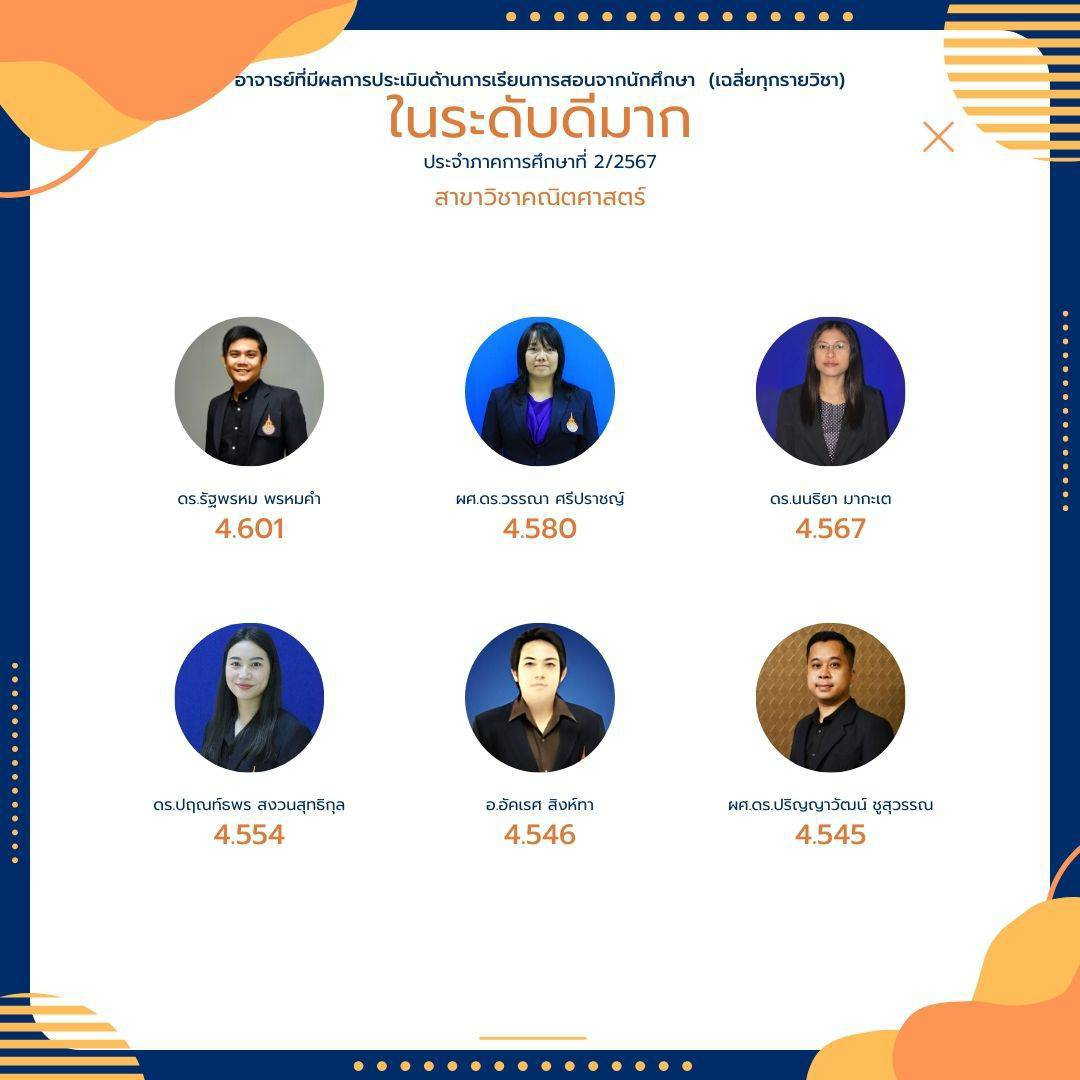
\includegraphics[width=0.6\textwidth]{Pic5.8-2.jpg}
	\caption{อาจารย์ที่มีผลการประเมินด้านการเรียนการสอนจากนักศึกษา (เฉลี่ยทุกรายวิชา)}
	\label{Pic5.8-2}
	\end{center}
\end{figure}
\newpage
\begin{doclist}
	\docitem{แนวทางการประเมินผลการปฏิบัติงานบุคลากรสายวิชาการคณะวิทยาศาสตร์และเทคโนโลยี}
	\docitem{เกณฑ์รางวัลสมนาคุณการตีพิมพ์บทความวิจัย}
	\docitem{ภาพแสดงความยินดีผ่านเว็บไซต์คณะ/Facebook ของสาขาวิชา}
\end{doclist}